\pagestyle{fancy}
\rhead{\bfseries OCR A-Level Computer Science}
\chead{\mdseries \thepage}
\lhead{\bfseries Jonathan Kasongo \mdseries — May 2025/26}
\lfoot{\sffamily Candidate number: N/A}
\rfoot{\sffamily Centre number: N/A}

\usetikzlibrary{positioning}
\usetikzlibrary{calc}

\chapter{Design}

\section{Breaking the problem down}
\label{sec:breakdown}

\textit
{
We now provide a simple visual decomposition of the problem at 
hand. We let DB denote our database for typographical reasons.
}

\begin{figure}[h]
\centering

\begin{tikzpicture}[every node/.style={scale=0.54}]

  \node[draw, rectangle, minimum width=4cm, minimum height=1cm, fill=lightestgray]
  (home) {\large \circled{1} Home page};

  \node[draw, rectangle, minimum width=4cm, minimum height=1cm, below=of home ]
    (login) {\large \circled{3} Login page};

  \node[draw, rectangle, minimum width=4cm, minimum height=1cm, below right=of home]
    (docs) {\large \circled{4} Documentation};

  \node[draw, rectangle, minimum width=4cm, minimum height=1cm, below left=of home]
    (help) {\large \circled{2} Help page};

  \node[draw, diamond, aspect=2, below=of login ]
    (new) {\large First time user?};

  \node[draw, rectangle, minimum width=4cm, minimum height=1cm, below left=of new ]
    (acc) {\large \circled{4} Create account};

  \node[draw, rectangle, minimum width=4cm, minimum height=1cm, below=of acc ]
    (add) {\large \circled{6} Add account to \textit{DB}};

  \node[draw, rectangle, minimum width=4cm, minimum height=1cm, below right=of new ]
    (back) {\large \circled{5} Log back in};

  \node[draw, rectangle, minimum width=4cm, minimum height=1cm, below=of back ]
    (main) {\large \circled{7} Main page};

  \node[draw, rectangle, minimum width=4cm, minimum height=1cm, below right=of main ]
    (join) {\large \circled{10} Join call page};

  \node[draw, rectangle, minimum width=4cm, minimum height=1cm, below=of join ]
    (code) {\large \circled{15} Enter passcode};

  \node[draw, diamond, aspect=2, minimum width=4cm, minimum height=1cm, below=of code ]
    (valid) {\large Is code valid?};

  \node[draw, rectangle, minimum width=4cm, minimum height=1cm, below left=of valid ]
    (codegood) {\large \circled{17} Connect to call};

  \node[draw, rectangle, minimum width=4cm, minimum height=1cm, below right=of valid ]
    (codebad) {\large \circled{18} Raise error};

  \node[draw, rectangle, minimum width=4cm, minimum height=1cm, below=of main ]
    (create) {\large \circled{9} Create call page};

  \node[draw, rectangle, minimum width=4cm, minimum height=1cm, below=of create ]
    (invite) {\large \circled{14} Invite others};

  \node[draw, rectangle, minimum width=4cm, minimum height=1cm, below left=of main ]
    (settings) {\large \circled{8} Settings page};

  \node[draw, rectangle, minimum width=4cm, minimum height=1cm, below left=of settings ]
    (video) {\large \circled{12} Video settings};

  \node[draw, rectangle, minimum width=4cm, minimum height=1cm, below=of settings ]
    (access) {\large \circled{13} Accessibility settings};

  \node[draw, rectangle, minimum width=4cm, minimum height=1cm, left=of video ]
    (audio) {\large \circled{11} Audio settings};

  \node[draw, rectangle, minimum width=4cm, minimum height=1cm, below=of video ]
    (save) {\large \circled{16} Save settings to \textit{DB}};

  \coordinate[right=2cm of code.east] (here);

  \coordinate[below=1.26cm of access.south] (a);

  \coordinate[below=1.26cm of audio.south] (b);

  \draw[black, -{Latex[length=2.5mm]}] 
    (home) -- (login);

  \draw[black, -{Latex[length=2.5mm]}] 
    (home) -| (docs);

  \draw[black, -{Latex[length=2.5mm]}] 
    (home) -| (help);

  \draw[black, -{Latex[length=2.5mm]}] 
    (login) -- (new);

  \draw[black, -{Latex[length=2.5mm]}] 
    (new) -| node[above] {Yes} (acc);

  \draw[black, -{Latex[length=2.5mm]}] 
    (new) -| node[above] {No} (back);

  \draw[black, -{Latex[length=2.5mm]}] 
    (acc) -- (add);

  \draw[black, -{Latex[length=2.5mm]}] 
    ([yshift=0.25cm]add) -| (new);
  
  \draw[black, -{Latex[length=2.5mm]}] 
    (back) -- (main);

  \draw[black, -{Latex[length=2.5mm]}] 
    (back) -- (main);

  \draw[black, -{Latex[length=2.5mm]}] 
    (main) -| (join);

  \draw[black, -{Latex[length=2.5mm]}] 
    (join) -- (code) ;

  \draw[black, -{Latex[length=2.5mm]}] 
    (code) -- (valid) ;
 
  \draw[black, -{Latex[length=2.5mm]}] 
    (valid) -| node[above] {Yes} (codegood) ;

  \draw[black, -{Latex[length=2.5mm]}] 
    (valid) -| node[above] {No} (codebad); 

  \draw[black, -{Latex[length=2.5mm]}] 
    ([xshift=0.4cm]codebad.north) -- (here) -- (code.east); 
  
  \draw[black, -{Latex[length=2.5mm]}] 
    (main) -- (create) ;

  \draw[black, -{Latex[length=2.5mm]}] 
    (create) -- (invite) ;

  \draw[black, -{Latex[length=2.5mm]}] 
    ([yshift=-0.25cm]main) -| (settings);

  \draw[black, -{Latex[length=2.5mm]}] 
    (settings) -- (access);

  \draw[black, -{Latex[length=2.5mm]}] 
    (settings) -| (video);

  \draw[black, -{Latex[length=2.5mm]}] 
    (settings) -| (audio);

  \draw[black, -{Latex[length=2.5mm]}] 
    (video) -- (save);

  \draw[black, -{Latex[length=2.5mm]}] 
    (audio.south) -- (b) -- (save.west);

  \draw[black, -{Latex[length=2.5mm]}] 
    (access.south) -- (a) -- (save.east);

\end{tikzpicture}

\caption{Decomposition of the problem.}
\label{fig:decomp}
\end{figure}

\subsection*{Explaining and justifying the breakdown}

As discussed in \ref{sec:computational} decomposition can 
reduce the complexity of a system by providing clear sub-tasks
that need to be achieved in order to solve a larger more 
complicated task. Moreover this method of organising tasks 
motivates a more modular approach to the implementation of our
system; each one of the main sub-tasks is neatly and clearly 
visualised and the overall presentation shows how each
sub-task relates to the others. \\ \vspace{0.2cm}

Starting from the top of the diagram I chose to display a
home page once the user initially accesses our website. The 
home page will be primarly used to greet the user, show them 
what the web-app can do and get them to login. However from
the home page users will also be able to access the system 
documentation as well as a help page if users are having issues
with using the system. We justify the need for a homepage by 
highlighting the importance of a first impression. A 
well-designed homepage can capture the attention of the user
and encourage them to explore the rest our web-app. If the
homepage is able to provide a good first impression we will be
able to garner a larger userbase, and simultaneously ensure an 
excellent user experience as they move around the UI. Moreover
if our users are satisfied then our client will be too. 
Documentation for the system will also be freely available to 
find on the the home page to be easily accessible for
developers. Furthermore the inclusion of the documentation 
on the home page means that developers aren't forced to create
an account just to read the documentation, saving much time for
these users. In this manner the system becomes entirely 
\textit{self-contained}, that is no other external resources 
would be necessary in order to use, maintain or update the
system. Finally in the case that users are experiencing issues
with the software a help page will also be clearly available on
the home page in order to answer FAQs as well as guide the user
through any troubleshooting. \\ \vspace{0.2cm}

The next pages require the user to first login. Upon entering 
the login page the user will be asked whether this is their 
first time using our system and if so they will be prompted to 
create an account. If it isn't the user's first time on our 
application then they will enter their username and password
and login to their account. The reason that we ask the user to 
login is because we would like each user to video conference 
with the settings that are most comfortable for them, once the
user logs in we can apply their specific accessibility 
settings that are tied to their account. Therefore in asking
the user to login before they begin video conferencing we are 
encouraging the user to take full advantage of our software by 
allowing them to first, adjust the settings to match their 
needs and requirements. \\ \vspace{0.2cm}

Once the user has logged in they will have complete access to 
the entire functionality of our web-app. I decided to seperate
the main content of the system into 3 pages, 1) Settings page,
2) Create call page, 3) Join call page. I chose to split the 
application into 3 main pages so that users won't have to 
search the app through one long overcrowded page in order to 
find what they are looking for. With this system users will be
able to quickly navigate to the page that they need and find 
what they are looking for easily on that page. Additionally, 
the concept of splitting our content onto multiple pages is 
easily scalable, if the site is updated and more content is 
added the developers can simply add a new page onto the site.
Consequently the system can rapidly expand in order to 
accommodate the growing number of user demands without
requiring a full website re-design each time an update is 
made. \\ \vspace{0.2cm}

The settings page will be where all the configurations and 
options for our system can be set/changed. It will be split
into 3 main tabs; the audio tab, the video tab and the 
accessibility tab. Each tab will hold settings related to it's
name that is, the audio tab will hold settings related volume
and sound and etc. Once a user makes some changes to any of the
settings their changes will be saved to their account and this 
data will remain on the database. The descision to split 
settings into 3 main tabs not only improves the user experience
by allowing users to find the settings they are looking for
easily but it's also in harmony with one of my client's main 
requests for this project; to have a \textit{"focus on 
simplicity"}. The descision to have settings for our system
will help each user to tailor their video conferencing
experience to fit to their personal needs. This allows us to 
create 1 system that is able to accommodate for a large 
number of people enhancing the accessibility of our platform, 
a request outlined by my client in \ref{sec:interview}. 

\subsection{Navigation via speech to text}

Suppose that we have a user that is blind or has some form 
of visual impairment. How would they use the system? Though 
these people may have limited vision, we often find that 
their other senses are heightened \cite{blind}. The person's
sense of touch, smell, hearing or taste may be better in order
to make up for the lack of vision. To allow our visually 
impaired users to be able to navigate the system comfortably 
we make use of their improved sense of hearing by allowing the
user to talk to the system in order to navigate to different 
pages and perform various actions. In implementing this 
feature we prevent the alienation of visually impaired users
by designing a system that allows them to be able to video
conference when they perhaps couldn't have before. This will 
not only expand our potential user base but it could also 
help these people to connect with others, by creating more 
opportunities for social interactions. Moreover 
we directly achieve one of the client's requests to create 
an \textit{accessible} video conferencing system. \\
\vspace{0.2cm}

One approach to the implementation of this feature could
be to have a set of phrases that we recognise as commands 
for the system, once 
the user says one of these commands our system should
recognise this and perform the corresponding action. An 
alternative may be to use some form of machine learning in 
order to process the user's speech and use natural language
processing to determine the user's intentions. This method is
arguably easiser for the user, instead of memorise some set
phrases for commands they can simply talk normally and the
system would recognise what the user would like to do. 
Although this approach may seem more attractive it is not 
without it's downsides. It is well known that machine 
learning is not perfect and that it can make mistakes from 
time to time. In this case the system making mistakes and
performing the wrong actions for the user could be extremely
confusing since the user may believe that they are on a
different webpage to the one that they actually are on. Since 
the model would have to pick up on a few very specific
commands in the user's speech it is unlikely that datasets 
would exist in order for us to use for the training of our 
machine learning model. Collecting the data on 
which to train the model on may be very time consuming for me.
Considering all of the downsides mentioned it seems 
reasonable to go with the safer option and use the set
phrases approach. In order to combat the potential problem of
having the system misunderstand the user's command we could 
make the user confirm their command before it is executed.
The system would read out the command that it has detected and
then the user could say "confirm" or "cancel" in order to 
go through with the action or stop the action respectively. 
Finally in the case that the user forgets what they have to 
say in order to perform an action they can say "help" to be 
reminded of these set phrases.
\\ \vspace{0.2cm}

We also need a method to actually recognise the user's speech.
As justified in the previous paragraph this method will need
to recognise certain set phrases and identify them correctly.
Mozilla firefox offers a Web speech API that implements 
features such as speech recognition, speech synthesis, and
speech to text. We could make use of their speech recognition
to turn their voice into text and then compare the text
produced to a each of the set phrases that we chose. Using an
API to implement this feature ensures that the speech recognition
code is robust and efficient as API's from large and reputable
companies are thoroughly tested. The use of an API also 
improves the maintainability of the software. Since the
implementation of the web speech functions has been abstracted 
away from the developer, the code is simpler, shorter and easier
to understand. We are able to directly benefit one of our
stakeholders, the IT staff (see section \ref{sec:stakeholders}),
through making the code clear and easy to understand.\\ \vspace{0.2cm}

To briefly summarise our research, we will make use of Mozilla
firefox's Web speech API to enable people with low vision to be 
able to navigate our system using their voice. In order to navigate
the system the user will say one of the set phrases, after which the 
system will repeat the phrase that it has heard and ask the user 
to confirm. If the user happens to forget which phrase to say in 
order to perform a certan action they may say "help" in order to 
hear a list of all of the set phrases and their actions.

\subsection{Defining the structure of the solution}

\subsubsection{Entity relationship diagram — \textit{1st draft}}
\label{sec:erdd}

% We need to store user logins, 
% user configurations say video, audio and accessibility 
% so 3 tables, one with logins, one with configurations, 
% etc... 

\textit{The acronym "cfg" denotes configuration.}

\begin{figure}[H]
\centering

\begin{tikzpicture}

  \pic{entity={logins}{\sffamily Logins}{
    \underline{UserID} & \texttt{int} \\
    Username & \texttt{string} \\
    Password & \texttt{string} \\
  }};

  \pic[below right=of logins]{entity={video}{\sffamily Video\_cfg}{
    \textit{UserID} & \texttt{int} \\
    Video quality & \texttt{int} \\
    Video on by default & \texttt{bool} \\
  }};

  \pic[below left=of logins]{entity={audio}{\sffamily Audio\_cfg}{
    \textit{UserID} & \texttt{int} \\
    Speaker volume & \texttt{int} \\
    Mic volume & \texttt{int} \\
    Mic on by default & \texttt{bool} \\
    Hide self-view & \texttt{bool} \\
  }};

  \pic[below=of logins]{entity={access}{\sffamily Accessibility\_cfg}{
    \textit{UserID} & \texttt{int} \\
    Font size & \texttt{int} \\
    Macros & \texttt{string} \\
  }};

  \draw[] (logins) -| (video);
  \draw[] (logins) -| (audio);
  \draw[] (logins) -- (access);

\end{tikzpicture}

\caption{The 1st draft ER diagram.}
\label{fig:erdd}
\end{figure}

% config id so that configs that are the same use same id

\textit{Explaining and justifying the 1st ER diagram draft.}
This entity relationship (ER) diagram was my first attempt at
designing the database for this project. It captures the 
general structure and idea that I had in mind for how the
database of my system should work. Loosely there are 4 main 
categories of data, login data, audio configurations,
video configurations and accessibility configurations, that
would have to be stored in our database. Naturally I decided 
to split these 4 categories into 4 individual tables, such 
that each table should hold 1 category of data. This should 
make life simpler once I begin implementation, for example 
when I have to make a queries about a collection of related
pieces of data I will only need to query the 1 table whose 
label should cover the data I need at that point. I make use 
of a unique numeric ID in order to identify each user and this
is seen as the primary key in the table {\sffamily Logins}.
These IDs are then used to link each user account to their 
relevant configurations via the 3 tables ending in 
{\sffamily \_cfg}. Though this design choice was ok for a 
first draft I soon realised that there were obvious
improvements that could be made. I present some of the flaws
of our current design with an illustration. Suppose that you 
wish to find \emph{all} the configurations that a specific 
user has tied to their account.

\begin{algorithm}
\caption*{\textbf{Algorithm} Pseudo code for finding all 
configurations tied to a user.}
\label{alg:long}
\sffamily

\begin{algorithmic}[1]
  \Function{Get\_All\_Configs}{ID}
    \Let{User\_ID}{ID}
    \Let{Configs}{$[]$} \Comment{Let Configs be an array.}
    \State{}
    
    \State{Configs.insert( Query\_tbl(Audio\_cfg, User\_ID, Speaker volume) )}
    \State{Configs.insert( Query\_tbl(Audio\_cfg, User\_ID, Mic volume) )}
    \State{Configs.insert( Query\_tbl(Audio\_cfg, User\_ID, Mic on by default) )}
    \State{Configs.insert( Query\_tbl(Audio\_cfg, User\_ID, Hide self-view) )}
    \State{\ldots}
    \State{}

    \State{\textbf{return} Configs}
  \EndFunction
\end{algorithmic}

\end{algorithm}

\mdseries

The algorithm above shows a sketch of the algorithm
necessary to solve our problem in pseudo-code. Unfortunately
with our database approach this request is tedious and
inelegant. The function will call the \code{Query\_tbl()}
function 9 times! Not only will this function be slow, due to
the repeated queries to an external database, but it
also violates the DRY software development principle we are
adhering to, as discussed in \ref{sec:computational}. We now 
propose a solution to this issue that allows us to use at most
2 calls to the \code{Query\_tbl()} function.

\subsubsection{Entity relationship diagram — \textit{2nd draft}}

\begin{figure}[H]
\centering

\begin{tikzpicture}

  \pic{entity={logins}{\sffamily Logins}{
    \underline{UserID} & \texttt{int} \\
    \textit{ConfigID} & \texttt{int} \\
    Username & \texttt{string} \\
    Password & \texttt{string} \\
  }};

  \pic[below=of logins]{entity={configs}{\sffamily Configs}{
    \underline{ConfigID} & \texttt{int} \\
    \textit{VideoID} & \texttt{int} \\
    \textit{AudioID} & \texttt{int} \\
    \textit{AccessID} & \texttt{int} \\
  }};

  \pic[below right=of configs]{entity={video}{\sffamily Video\_cfg}{
    \underline{VideoID} & \texttt{int} \\
    Video quality & \texttt{int} \\
    Video on by default & \texttt{bool} \\
  }};

  \pic[below left=of configs]{entity={audio}{\sffamily Audio\_cfg}{
    \underline{AudioID} & \texttt{int} \\
    Speaker volume & \texttt{int} \\
    Mic volume & \texttt{int} \\
    Mic on by default & \texttt{bool} \\
    Hide self-view & \texttt{bool} \\
  }};

  \pic[below=of configs]{entity={access}{\sffamily Accessibility\_cfg}{
    \underline{AccessID} & \texttt{int} \\
    Font size & \texttt{int} \\
    Toggle mute & \texttt{int} \\
    Toggle camera & \texttt{int} \\
    {$\cdots$} & {$\cdots$} \\
  }};

  \coordinate[right=7.5em of configs.east] (v);
  \coordinate[left=7.5em of configs.west] (a);

  \draw[-{crow's foot}] (configs) -- (logins);
  \draw[-{crow's foot}] (audio.north) -| (a) -- (configs.west);
  \draw[-{crow's foot}] (access) -- (configs);
  \draw[-{crow's foot}] (video.north) -| (v) -- (configs.east);

\end{tikzpicture}

\caption{The 2nd draft ER diagram.}
\label{fig:erdf}
\end{figure}

\textit{Explaining and justifying the 2nd draft ER diagram.}
The dots in the {\sffamily Accessibility\_cfg} table indicate
that there are potentially more fields in this table. \\ \vspace{0.2cm}

The changes in the final ER diagram all revolve around the new
ConfigID attribute. The user's complete configuration used to 
be comprised of numerous attributes that were stored across
multiple tables. Now each collection of configuration
attributes has been given it's own table in the
{\sffamily Configs} table. This table stores a number of IDs
that each map to a collection of configuration attributes.
In essence instead of treating each configuration attribute as
it's own seperate object, we now store all of a user's 
configurations together in one object, like how a bag stores
a collection of items. This approach to our database design
allows us to solve the problem we had in \ref{fig:erdd}, now
in order to request \textit{all} of a user's configurations
we may use the following two-liner;\\

\begin{center}
\begin{tblr}{colspec={l}, rowsep=0pt}
  {\sffamily Config\_ID} $\gets$ {\sffamily Query\_tbl(Logins, UserID, ConfigID)}\\
  {\sffamily \textbf{return} Query\_tbl(Configs, Config\_ID)}\\
\end{tblr}
\end{center}

Not only is this code much shorter and more clear than the 
code in the algorithm above but it will also run much
faster, with just 2 calls to \code{Query\_tbl()}. Moreover
with this new approach we can still adhere to the DRY software
development principle, since we are no longer forced to repeat
code unnecessarily. The database is also in 3rd normal form
enhancing the efficiency of our system as 
well as ensuring that data integrity is achieved.
Another issue that this new design solves
is duplicate configurations. For instance in figure 
\ref{fig:erdd} if 2 users happen to have the same
configuration then this data will simply be duplicated in our 
table and take up unnecessary space in our table. However 
with the design in figure \ref{fig:erdf} if 2 users have for
example the same audio settings then they can simply use the
same audio ID, meaning that this specific audio configuration 
only needs to be stored once in our database. It is clear to 
see that with this new approach we not only save memory in 
the long term, at the cost of 1 extra table, but we also 
improve the performance of our system dramatically. \\
\vspace{0.2cm}

Although the
database system will increase in size temporarily I argue that
the size of the database will be smaller as compared to the 
draft database design as the number of users increases. All of
our configuration options take a discrete set of values, for 
instance font size will only be able to take on an integer
value $12 \leq f \leq 40$. For each configuration option let
$c_1, c_2, \ldots, c_N$ be the of length $N$ sequence of all
the possible configurations for our 
system (note that this is allowed because all of configuration
options are numerical, the \texttt{bool} data type can simply
be represented by a number that is either 0 or 1). Denote
$c_i$ to be the $i$-th configuration and $|c_i| \in \mathbb{N}$
to be the number of possible options that this configuration 
can take on. Suppose that we have $n$ users in our system,
for each configuration option let
$X_{i, 1}, X_{i, 2}, \ldots, X_{i, n}$ a sequence of $n$
independent discrete uniform random variables, 
where $X_{i, j}$ denotes the value of the $i$-th configuration
option for the $j$-th user. Let $\mu_i$ be the finite expected
value of the $i$-th configuration. Denote $\overline{X_i}$ to 
be the sample mean of the $i$-th configuration for all or our
$n$ users. By \textit{Kolmogorov's strong law} \cite{thm}
we have,

\begin{equation} \label{eq:kol}
  Pr \left(\lim_{n \to \infty} \overline{X_i} = \mu_i \right) = 1
\end{equation}

over all valid values of $i$. From the definition of a limit
we can conclude that as $n$ grows larger the sample mean 
converges almost surely to it's expected value. That means
that as the number of users increases, the likelyhood that 
users will choose the same configuration option increases 
significantly meaning the number of redundancies in our table 
increases significantly too. Whilst
equation \ref{eq:kol} can provide some motivation for the 
direction of our arguement \textit{Kolmogorov's strong law}
cannot be applied because we can never have an infinite number
of users in our system. Instead we will consider the
configuration option $c_m$ where this configuration option is
able to take on the largest number of values.\\ \vspace{0.2cm}

Formally, we
take a configuration option $c_m$ such that
$\max_{i=1}^{N} |c_i| = |c_m|$. We will then show that with a 
sufficiently large userbase that users will inevitably start
picking the same values for their configuration options. The 
options that are able to take on the largest number of values 
are the 2 volume options in {\sffamily Audio\_cfg}. We let 
users choose some integer volume $0 \leq v \leq 100$. By the 
\textit{pigeonhole principle} once we have 102 users we 
must have at least 2 users who have chosen the same 
volume $v$. This is because we have 101 different options for 
the value that $v$ could take on, and in the worst case 
scenario each user would take on a unique value of $v$. Above
the threshold of 101 users every value of $v$ would already 
have at least 1 user who has selected this value and hence the
$102^{nd}$ user has to choose a volume value which someone else
has already chosen. More generally starting from user 1, every
$101^{th}$ user must choose a volume that has already been 
chosen before causing a new duplicate. This is seen by 
repeatedly applying the \textit{pigeonhole principle}. As the
number of users increase the number of duplicates for volume
grows linearly. For instance if we have just 
$1011 = 101 \cdot 10 + 1$ users then we must
have at least 10 duplicates for values of $v$. More worryingly
since the volume example was the worst case scenario (because
volume has the largest number of options that a user can 
choose) we can see that every other configuration option will 
also have to have $\geq 10$ duplicates. We have 9 options 
total so across all tables there has to be at least 90
duplicates, and in fact the number of duplicates will be much 
greater in reality. The 4 boolean options will have
duplicates every 2 users! Hence these options will at least
505 duplicates (from the calculation $2 \cdot 505 + 1 = 1011$).
Multiplying by the 4 boolean options yields 2020 duplicates
\textit{minimum} over the 4 boolean options only! It is not 
hard to see that once the number of users starts to grow our
database will rapidly fill up with duplicates resulting in
catastrophically large database sizes and hence users will be
unable to use our system as their data simply can no longer  
recorded in our database. With our final database design we 
can guarantee that our database won't have any duplicates 
saving me and my client from a multitude of economical and 
logistical issues in the future. \\ \vspace{0.2cm}
%mumble mumble Central limit thm, lots of collisions mumble 

\subsubsection{Entity relationship diagram — \textit{3rd draft}}

\begin{figure}[H]
\centering

\begin{tikzpicture}

  \pic{entity={logins}{\sffamily Logins}{
    \underline{UserID} & \texttt{int} \\
    \textit{AudioID} & \texttt{int} \\
    \textit{AccessID} & \texttt{int} \\
    \textit{VideoID} & \texttt{int} \\
    Username & \texttt{string} \\
    Password & \texttt{string} \\
  }};

  \pic[below right=of logins]{entity={video}{\sffamily Video\_cfg}{
    \underline{VideoID} & \texttt{int} \\
    Video quality & \texttt{int} \\
    Video on by default & \texttt{bool} \\
  }};

  \pic[below left=of logins]{entity={audio}{\sffamily Audio\_cfg}{
    \underline{AudioID} & \texttt{int} \\
    Speaker volume & \texttt{int} \\
    Mic volume & \texttt{int} \\
    Mic on by default & \texttt{bool} \\
    Hide self-view & \texttt{bool} \\
  }};

  \pic[below=of logins]{entity={access}{\sffamily Accessibility\_cfg}{
    \underline{AccessID} & \texttt{int} \\
    Font size & \texttt{int} \\
    Toggle mute & \texttt{int} \\
    Toggle camera & \texttt{int} \\
    {$\cdots$} & {$\cdots$} \\
  }};

  \coordinate[right=7.5em of configs.east] (v);
  \coordinate[left=7.5em of configs.west] (a);

  \draw[-{crow's foot}] (logins) -| (audio);
  \draw[-{crow's foot}] (logins) -- (access);
  \draw[-{crow's foot}] (logins) -| (video);

\end{tikzpicture}

\caption{The 3rd ER diagram.}
\label{fig:erd3}
\end{figure}

\textit{Explaining and justifying the 3rd ER diagram.} We
will first explain the shortcomings of the 2nd database
design and then explain how the 3rd design was created in 
order to resolve these issues. The intention in creating the 
ConfigID key was to provide a clearer and more organised way
to store data on the user's configuration options. In this way 
we wouldn't have to set up queries that ask for the value
each option individually, we could instead simply query for the 
ID of the category of configuration we would like 
(audio, accessibility or video) and then use an object to store
all the attributes in that category and their corresponding values.
This means that we will reduce the number of queries that we would
need to make to the database, improving the performance of our 
application. Additionally through employing this approach to the 
database design we make the configuration system more modular. 
Indeed if 2 users happen to have the same accessibility
configurations then instead of storing a duplicate entry in our
table the users can simply use the same AccessID. \\ \vspace{0.2cm}

Suppose that a user would like to change their configuration. 
How would we know whether this configuration is already taken,
(so we should give this user the same ConfigID as the one already 
found in the database) or whether this configuration is new 
(so we should give this user a new unique ConfigID). The most
obvious naive solution would be to iterate over all configurations
checking whether or not configuration is the same as the one created
by the user. Since different ConfigID's may have the same AudioID 
or the same VideoID, and etc \footnote{Only 1 of the AccessID,
AudioID, VideoID has to be different in order to create a new
ConfigID.}, we will spend a lot of time performing redundant
checks. Let's reinforce this arguement using a concrete example,
suppose that the 2 ConfigID's \texttt{001} and \texttt{002} are set up like so.

\begin{center}
\begin{tblr}{cccc}
  \hline
  ConfigID & AudioID & VideoID & AccessID \\
  \hline
  \texttt{001} & \texttt{521} & \texttt{126} & \texttt{078} \\
  \texttt{002} & \texttt{521} & \texttt{126} & \texttt{024} \\
\end{tblr}
\end{center}

Clearly the 2 configurations are exactly the same apart from 
their different accessibility settings. Now imagine that 
another user changes their configuration. We first check 
whether or not this user's configuration is the same as
ConfigID \texttt{001}. We check all the attributes in Audio
config \texttt{521} then all attributes in Video config
\texttt{126} and then all the attributes in Accessibility config
\texttt{078}. Suppose that the configurations happened to be 
different. We now have to check whether or not this user's 
configuration is the same as ConfigID \texttt{002}. We check 
again check all the attributes in Audio config \texttt{521},
then all the attributes in Video config \texttt{126} and then
all the attributes in Accessibility config \texttt{024}. Now 
the problem is clear: we have checked over the same audio and 
video configuration twice! This is a huge waste of resources and 
the issue will become worse as more user configs are added to 
the database. \\ \vspace{0.2cm}

The solution: to remove the ConfigID attribute. In studying this 
example we will find that the ConfigID attribute is unnecessary.
Although it's addtion was intended to provide clarity and
organisation it ended up creating redundancies and needlessly
complicating the system. Now in order to solve the problem of 
changing a user's configuration we can simply do checks against
all audio configs, then all video configs and then all
accessibility configs. Through this approach we know that each 
of the configs that we check is unique, and we ultimately avoid 
the downfall of the 2nd database draft, redundancies. 

\subsubsection{Entity relationship diagram — \textit{4th draft}}

\begin{figure}[H]
\centering

\begin{tikzpicture}

  \pic{entity={logins}{\sffamily Logins}{
    \underline{UserID} & \texttt{int} \\
    \textit{AudioID} & \texttt{int} \\
    \textit{VideoID} & \texttt{int} \\
    \textit{AccessID} & \texttt{int} \\
    Username & \texttt{string} \\
    Password & \texttt{string} \\
  }};

  \pic[below right=of logins]{entity={video}{\sffamily Video\_cfg}{
    \underline{VideoID} & \texttt{int} \\
    Video quality & \texttt{int} \\
    Video on by default & \texttt{bool} \\
    {$\cdots$} & {$\cdots$} \\
  }};

  \pic[below left=of logins]{entity={audio}{\sffamily Audio\_cfg}{
    \underline{AudioID} & \texttt{int} \\
    Speaker volume & \texttt{int} \\
    Mic volume & \texttt{int} \\
    Mic on by default & \texttt{bool} \\
    Hide self-view & \texttt{bool} \\
    {$\cdots$} & {$\cdots$} \\
  }};

  \pic[below=of logins]{entity={access}{\sffamily Accessibility\_cfg}{
    \underline{AccessID} & \texttt{int} \\
    Font size & \texttt{int} \\
    Toggle mute & \texttt{int} \\
    Toggle camera & \texttt{int} \\
    {$\cdots$} & {$\cdots$} \\
  }};

  \coordinate[left=13.6em of logins.west] (v);
  \coordinate[above=0.4cm of v] (al);

  \coordinate[left=1.45em of logins] (p);
  \coordinate[below=0.5cm of p] (acl);

  \coordinate[right=1.45em of logins] (j);

  \draw[-{crow's foot}] ([yshift=1.5cm]audio.west) -| (al) -- ([yshift=0.4cm]logins.west);
  \draw[-{crow's foot}] ([yshift=1cm]access.west) -| (acl) -- ([yshift=-0.5cm]logins.west);
  \draw[-{crow's foot}] ([yshift=1cm]video) -| (j) -- (logins);

\end{tikzpicture}

\caption{The 4th ER diagram.}
\label{fig:erd4}
\end{figure}

\textit{Explaining and justifying the 4th ER diagram.} 
In the 4th draft, the manner in which we have presented 
the database design has changed due to requests from my 
client. Each primary to foreign key relationship
is now represented with an arrow that points directly to 
to the name of it's corresponding key. Moreover the 
logical relationships between attributes have been 
corrected.

\subsubsection{Proposed system level 0 DFD}

\begin{figure}[H]
\label{fig:dfd0}
\centering
\begin{tikzpicture}

  \node[draw, rectangle, minimum width=4cm, minimum height=1cm,
	fill=lightestgray]
    (sys) {\large Proposed system};

  \node[draw, ellipse, minimum width=3cm, minimum height=1.5cm,
	below right=of sys]
    (user) {\large Users};

  \node[draw, ellipse, minimum width=3cm, minimum height=1.5cm,
	below left=of sys]
    (host) {\large Host};

  \node[draw, ellipse, minimum width=3cm, minimum height=1.5cm,
	above=of sys]
    (main) {\large Maintainers};

  \coordinate[below=1cm of sys.north] (A);

  \draw[black,  -{Latex[length=2.5mm]}]
	  (sys) edge["1"] (main);
  \draw[black, bend left=0.5cm, -{Latex[length=2.5mm]}]
	  (host) edge["2"] (sys);
  \draw[black, bend left=0.5cm, -{Latex[length=2.5mm]}]
	  (sys) edge["3"] (host);
  \draw[black, bend left=0.5cm, -{Latex[length=2.5mm]}]
	  (sys) edge["3"] (user);
  \draw[black, bend left=0.5cm, -{Latex[length=2.5mm]}]
	  (user) edge["4"] (sys);

  \draw[black, bend left=1.75cm, -{Latex[length=2.5mm]}]
          (A) edge["5"] (host);
  \draw[black, bend right=1.75cm, -{Latex[length=2.5mm]}]
          (A) edge["5"] (user);
\end{tikzpicture}

\caption{Proposed system level 0 DFD diagram.}
\end{figure}

\textit{An explanation of the DFD is found below. The number 
closest to each edge refers to the number in the left column
of the explanation table below.} \vspace{-0.2cm}

%recieve feedback from users
\begin{longtblr}[
  caption={Explanation of proposed system DFD.}
]{
  colspec={lX}, hlines, row{1}={lightestgray}
}

Edge & Commentary \\

1 & {Maintainers recieve and analyse information relating to 
     the performance of the proposed system, and use the
     documentation provided with the system to suggest and 
     make any necessary changes.} \\

2 & {The host uses the proposed system in order to commence
     video conferences and to invite all those whom they would
     like to. Moreover the host will use the system to admit 
     or remove people from the video conference, as they 
     wish.} \\

3 & {The system provides the host with live audio and video 
     from all the other participants in the video conference,
     provided their microphone or camera are connected and that
     the user has activated their microphone or camera from
     their end.}\\

4 & {The user connects to video conferences via a code that 
     was given to them by the host of the meeting. They can 
     also raise their hand and tailor their experience via
     the settings page.}\\

5 & {Hosts and users are both able to communicate either via 
     their microphones or via the built-in chat box on every 
     video conference.}\\
  
\end{longtblr}

\textit{Justifying the DFD.} The DFD above allows me and my 
client to be able to clearly understand the plans for the 
proposed system, in terms of some of it's main features and 
functionalities. Furthermore the DFD diagram can be compared to
the previous system's DFD diagram to ensure that the new 
system is an adequate replacement, as discussed in
\ref{sec:currdfd}. The usage of primitive shapes and clear 
labelling ensures that the diagram is easily digestible, such 
that even those who don't understand anything about software
architecture will be able to grasp the structure of the 
proposed solution. Consequently these diagrams also work to 
improve the maintainability of the system, even new developers
with minimal programming experience will have an intuitive 
understanding of how the proposed system works and it's
overarching structure. Hence thanks to the creation of these 
diagrams we do not only equip the future maintainers of this 
system with all the necessary understanding that they require
to make changes, but we also promote a design culture of clear
and maintable software. Then if the future maintainers of this
software feel motivated to do the same we can ensure that our 
software will maximise it's longevity, through the constant 
innovation and improvement of our system namely via it's 
future maintainers.

\subsubsection{Proposed system level 1 DFD} 

\begin{figure}[H]
\centering

\begin{tikzpicture}

\node[draw, rectangle, minimum width=2.8cm, minimum height=1cm,
      fill=lightestgray]
  (logins) {Logins};

\node[draw, rectangle, minimum width=2.8cm, minimum height=1cm,
      below=of logins, fill=lightestgray]
  (access) {Accessibility};

\node[draw, rectangle, minimum width=2.8cm, minimum height=1cm,
      below left=of logins, fill=lightestgray]
  (audio) {Audio};

\node[draw, rectangle, minimum width=2.8cm, minimum height=1cm,
      below right=of logins, fill=lightestgray]
  (video) {Video};

\node[draw, rectangle, minimum width=2.8cm, minimum height=1cm,
      below=of access, fill=lightestgray]
  (docs) {Documentation};

\node[draw, ellipse, minimum width=2.8cm, minimum height=1cm,
      above=10cm of logins]
  (user) {Users};

\node[draw, ellipse, minimum width=2.8cm, minimum height=1cm,
      above=12cm of audio]
  (it) {Maintainers};

\node[draw, ellipse, minimum width=2.8cm, minimum height=1cm,
      above=12cm of video]
  (host) {Host};

\coordinate[left=2.4cm of logins]  (a);
\coordinate[right=2.4cm of logins] (v);
\coordinate[below=3.5cm of host] (p);
\coordinate[above=3.5cm of logins] (qp);
\coordinate[left=3.5cm of qp] (q);
\coordinate[below=3.5cm of user] (rp);
\coordinate[left=3.5cm of rp] (r);
\coordinate[below=2cm of user] (d);
\coordinate[above=4cm of audio] (s);
\coordinate[left=4cm of docs] (l);
\coordinate[above=4cm of l] (u);

\draw[-{crow's foot}] (access) -- (logins);
\draw[-{crow's foot}] (audio) -- (a) -- (logins);
\draw[-{crow's foot}] (video) -- (v) -- (logins);

\draw[black, -{Latex[length=2.5mm]}] ([yshift=1.5cm]p) -| ([xshift=2cm]user);

\draw[black, -{Latex[length=2.5mm]}]
  (docs) --  (l) -- (u) -- node[rectangle split, rectangle 
                  split parts=2, text height=1.0ex, 
		  text width=7.5em, text centered,
		  fill=white] 
        {\nodepart[font=\scriptsize]{second}
	\begin{tblr}{colspec={X},vlines,hlines}
	\texttt{O} \hspace{0.1cm} \vline \hspace{0.1cm} Download\\
        Maintainers can download the documentation\\
        \end{tblr}} (s) -- (it);

\draw[black, -{Latex[length=2.5mm]}]
  (user) -- node[rectangle split, rectangle 
                  split parts=2, text height=1.0ex, 
		  text width=7.5em, text centered,
		  fill=white] 
        {\nodepart[font=\scriptsize]{second}
	\begin{tblr}{colspec={X},vlines,hlines}
	\texttt{I} \hspace{0.1cm} \vline \hspace{0.1cm} Registers\\
        User registers a new account on our system\\
        \end{tblr}
        } (logins);

\draw[black, -{Latex[length=2.5mm]}]
  (video) -- node[rectangle split, rectangle 
                  split parts=2, text height=1.0ex, 
		  text width=7.5em, text centered,
		  fill=white] 
        {\nodepart[font=\scriptsize]{second}
	\begin{tblr}{colspec={X},vlines,hlines}
	\texttt{P} \hspace{0.1cm} \vline \hspace{0.1cm} Audio \& video\\
        {Audio and video from other users is taken and processed 
	then sent to all other participants}\\
        \end{tblr}
        } (p) -- node[rectangle split, rectangle 
                  split parts=2, text height=1.0ex, 
		  text width=7.5em, text centered,
		  fill=white] 
        {\nodepart[font=\scriptsize]{second}
	\begin{tblr}{colspec={X},vlines,hlines}
	\texttt{O} \hspace{0.1cm} \vline \hspace{0.1cm} Audio \& video feeds\\
        {Audio and video from other users is output to all other participants}\\
        \end{tblr}} (host);

\draw[black, -{Latex[length=2.5mm]}]
  (user.south) -- (d) -| (r) -| node[rectangle split, rectangle 
                  split parts=2, text height=1.0ex, 
		  text width=7.5em, text centered,
		  fill=white] 
        {\nodepart[font=\scriptsize]{second}
	\begin{tblr}{colspec={X},vlines,hlines}
	\texttt{I} \hspace{0.1cm} \vline \hspace{0.1cm} Passcode\\
        User enters passcode to log back in\\
        \end{tblr}} (q) -| ([xshift=-5cm]logins);

\end{tikzpicture}

\caption{Proposed system level 1 DFD diagram.}
\label{fig:l1}
\end{figure}

\textit{The DFD is explained via the dialog boxes in 
the figure above}.\\ \vspace{0.2cm}

\textit{Justifying the DFD.} The level 1 data flow diagram 
exists to present a more in-depth look at the functionality of
the proposed system, specifically in regards to the inputs and 
outputs of the system. Additionally the level 1 DFD diagram can help 
us to get a general understanding of the various inputs and 
outputs that our software will have to produce. Through these
diagrams we can layout and clearly view the structure and
design of our system holistically and see how each component
of our system links to and integrates in with the other components.
Moreover data flow diagrams can also help us in the testing our 
software. Through a study of the diagram we can notice that the
figure \ref{fig:l1} acts a guide for the expected inputs and
outputs (I/O) of our system, which we can use to compare against
the actual I/O of our system during the development process.
Indeed the level 1 DFD coupled with the problem decomposition 
diagram serve as the "blueprints" of our system, visually 
illustrating the structure of our proposed system in a manner 
that is clear and simple to understand for both me and my client 
to refer to in the future.
Finally we have seen that the level 1 DFD diagram provides a
neat, cohesive visual representation of our system's architecture.

\subsection{Key algorithms}

% Use appropiate and accurate algorithms, justifying how these
% algorithms justifying how these algorithms form a complete
% solution to the problem.

% Identified and justified any further data to be used in the
% post development phase.

\textbf{Note:} \textit{The boxed number in front of each subheading refers 
to the corresponding boxed number found in the system 
decomposition in \ref{fig:decomp}.}

\subsubsection{\circled{6} Account creation}

\begin{tblr}{colspec={lX}, row{1}={lightestgray}}

\textit{Function name:} & {\scshape Add\_Account}(\texttt{string} {\sffamily Username}, \texttt{string} {\sffamily Password})\\

\textit{Description:}  & {This function will recieve in a username and password and add these details 
into the login table, provided that the username is not taken. We assume that the username and 
password have already been properly validated via the algorithm in the previous subheading. It returns
false if the username is taken and true if it is not.}\\

\textit{Justification:} & {Users need to create an account in order to be able to save their configurations.
For a detailed justification, refer to section \ref{sec:features}}\\

\end{tblr}

\begin{algorithm}
\caption{Pseudo code for creating a new user account.}
\sffamily

\begin{algorithmic}[1]
  \Function{Add\_Account}{Username, Password}
    \If{Query\_tbl(Logins, Username) $\neq$ \textbf{null}} \Comment{Cannot create account if username is taken.}
      \State{\textbf{return} False}
    \EndIf
    \State{}
   
    \State{Insert\_tbl(Logins, Username, Password, Default\_cfg)} \Comment{Set default settings for new user.}
    \State{}

    \State{\textbf{return} True}
  \EndFunction
\end{algorithmic}

\end{algorithm}
\mdseries

\textit{Iterative test plan: (These tests take place assuming that the logins table is empty each time)} \\ \vspace{0.2cm}

\begin{tblr}{colspec={lXXX}}

\hline

Test type & Input & Expected Output & Justification \\

\hline

Normal & \texttt{(TerryTao, re\%k91)} & \texttt{True} & {The 
system should correctly be able to add a new user.}\\

Erroneous & Call the function 2 times with this input \texttt{(TerryTao, re\%k91)} & \texttt{False} & {The
system should not be able to add a user that already exists.}\\

\hline

\end{tblr}


\subsubsection{\circled{4} Validate username and password}

\begin{tblr}{colspec={lX}, row{1}={lightestgray}}

\textit{Function name:} & {\scshape Validate\_Account}(\texttt{string} {\sffamily Username}, \texttt{string} {\sffamily Password})\\

\textit{Description:} & {This function will recieve in a username and password and check whether the
given password is strong enough and whether or not the username is acceptable. A username is considered
acceptable if it is at least 3 characters long, doesn't start with a special character, and only consists of 
the characters a-z, A-Z, 0-9, "\_" or "-". Function should return true if the given username and password are 
acceptable.}\\

\textit{Justification:} & {We should ensure that the user uses a strong password, and has a username that can be read. For 
instance if we had no restrictions on the username, the user could choose the username "\texttt{   }" which is obviously not 
readable, as it only consists of white spaces.}\\

\end{tblr}

\begin{algorithm}[H]
\caption{Pseudo code for validating a username and password.}
\sffamily

\begin{algorithmic}[1]
  \State{\textbf{import} zxcvbn}
  \Function{Validate\_Account}{Username, Password}
    \If{Username.length $<$ 3} 
      \State{\textbf{return} false}
    \EndIf

    \State{}
    \State{Pass\_strength $\gets$ zxcvbn(Password)}
    \State{Legal\_chars $\gets$ \{'a', 'b', 'c', $\ldots$\}} \Comment{Set of acceptable characters}
    \State{}
    \If{Pass\_strength.score $<$ 2} \Comment{Password is too weak}
      \State{\textbf{return} false}
    \EndIf

    \State{}
    \For{char \textbf{in} Username}
      \If{\textbf{not} char \textbf{in} Legal\_chars}
        \State{\textbf{return} false}
      \EndIf
    \EndFor
    
    \State{}
    \State{\textbf{return} true}
  \EndFunction
\end{algorithmic}

\end{algorithm}
\mdseries

\textit{Iterative test plan:}\\ \vspace{0.2cm}

\begin{tblr}{colspec={lXXX}}

\hline

Test type & Input & Expected Output & Justification \\

\hline

Normal & \texttt{("David\_Hilbert1", "i\#1Go8")} & \texttt{True} & {The
function should return true if the username fits the criteria stated and 
if the password is strong enough.}\\

Extreme & \texttt{("Dav", "i\#1Go8")} & \texttt{True} & {The 
function should still return true if the username given is 3 acceptable
characters.}\\

Erroneous & \texttt{("c", "123")} & \texttt{False} & {The function
should return false if the password is too weak and the username is not
considered acceptable.}\\

\hline

\end{tblr}

\subsubsection{\circled{5} Log user in}

\begin{tblr}{colspec={lX}, row{1}={lightestgray}}

\textit{Function name:} & {\scshape Log\_User\_In}(\texttt{string} {\sffamily Username}, \texttt{string} {\sffamily Password})\\

\textit{Description:}  & {This function should take in a user's username and password and then load in their relevant 
                          configurations. We should check that the password given matches the password stored in the database.
			  Their customised settings should all be correctly loaded into the system, once we have
			  confirmed that the user has successfully logged in. The function should return true if the user 
		          has successfully logged in and false if they have not.}\\

\textit{Justification:} & {The initiative to provide accessibility options and configurations was suggested by my client as a 
                           non-essential feature as was seen in section \ref{sec:interview}. Through providing our users with 
			   these options and configurations we enable them to customise their video conferencing experience so 
			   that their settings are tailor-made to suit their individual needs. We justify confirming that the
		           user has logged in by noting that in order for the user to be able to access their configurations 
		           we must know this user's UserID. Without the UserID we will not be able to query the database and 
		           therefore we won't be able to load their configurations.}\\

\end{tblr}

\begin{algorithm}[H]
\caption{Pseudo code for logging a user in.}
\sffamily

\begin{algorithmic}[1]
  \Function{Log\_User\_In}{Username, Password}
    
    \If{Query\_tbl(Logins, Username) $=$ \textbf{null}} \Comment{User doesn't exist.}
      \State{\textbf{return} False} 
    \EndIf

    \State{}

    \If{Query\_tbl(Logins, Username, Password) $\neq$ Password} \Comment{Wrong password.}
      \State{\textbf{return} False}
    \EndIf

    \State{}

    \Let{UserID}{Query\_tbl(Logins, Username, UserID)}
    \Let{Video\_ID}{Query\_tbl(Logins, UserID, VideoID)}
    \Let{Audio\_ID}{Query\_tbl(Logins, UserID, AudioID)}
    \Let{Access\_ID}{Query\_tbl(Logins, UserID, AccessID)}

    \State{}

    \State{Set\_Video(VideoID)}
    \State{Set\_Audio(AudioID)}
    \State{Set\_Access(AccessID)}

    \State{}

    \State{\textbf{return} True}
  \EndFunction
\end{algorithmic}

\end{algorithm}
\mdseries

\textit{Iterative test plan (These tests take
place assuming that the logins table only has
one account setup with the name 
\texttt{TestAcc1} and password \texttt{A2d£l!}):} \vspace{0.2cm} \\

\begin{tblr}{colspec={lXXX}}

\hline

Test type & Input & Expected Output & Justification \\

\hline

Normal & \texttt{(TestAcc1, A2d£l!)} & \texttt{True} & {The
system should function correctly when loading in a an actual
user's configurations with correct information.}\\

Extreme & \texttt{(TestAcc1, password)} & \texttt{False} & {The
system should recognise that the password inputted is incorrect
and should not allow the user to log in.}\\

Erroneous & \texttt{(kirishkiwi, password)} & \texttt{False} & {The
system should recognise that this user doesn't exist and should not
allow them to log in.}\\

\hline

\end{tblr}

\subsubsection{\circled{16} Update user settings}

\begin{tblr}{colspec={lX}, row{1}={lightestgray}}

\textit{Function name:} & {\scshape Set\_User\_cfgs}(\texttt{string} {\sffamily Username},
						     \texttt{string} {\sffamily Category},
	                                             \texttt{string} {\sffamily Option},
						     \texttt{int} {\sffamily Value})\\

\textit{Description:}  & {This function will update the user's current settings. If the given user 
	                  doesn't exist the function will return false. It will save
                          these changes to the database so that they can be retrieved later. If the 
		          specific configuration is already stored in the database than the user's 
		          config id will change to the id of the configuration already stored in the
		          database. Otherwise a new configuration id will be created and assigned to
		          the user.}\\

\textit{Justification:} & {By allowing the user to be able to save their customised settings we 
                           save them a deal of time. Users won't have to repetitively re-configure
		           their settings each time they log in, instead their settings are saved 
		           in our database to be loaded in. Since our target user base is the elderly
		           it is also likely that their memory is poor, by enabling these ones to 
		           set their configurations once and then have these settings be saved
			   automatically we also save them from having any issues remembering how to 
		           set up their config.}\\

\end{tblr}

\begin{algorithm}[H]
\caption{Pseudo code for updating a user's settings.}
\sffamily

\begin{algorithmic}[1]
  \Function{Set\_User\_cfgs}{Username, Category, Option, Value}
    \State{\textbf{If} Check\_User\_exists(Username) $\neq$ True: \textbf{return} False} \Comment{User doesn't exist.}
    \State{}
    
    \Let{UserID}{Query\_tbl(Logins, Username, UserID)}
    \Let{AudioID}{Query\_tbl(Logins, UserID, AudioID)}
    \Let{VideoID}{Query\_tbl(Logins, UserID, VideoID)}
    \Let{AccessID}{Query\_tbl(Logins, UserID, AccessID)}

    \State{}
    \Let{Audio\_cfg}{Create\_Audio\_cfg(AudioID)} \Comment{These are objects storing the user's current settings.}
    \Let{Access\_cfg}{Create\_Access\_cfg(AccessID)}
    \Let{Video\_cfg}{Create\_Video\_cfg(VideoID)}

    \State{}

    \State{\textbf{If} Category $=$ "Audio": Config $\gets$ Audio\_cfg} \Comment{Config is the configuration object being updated.}
    \State{\textbf{If} Category $=$ "Video": Config $\gets$ Video\_cfg}
    \State{\textbf{If} Category $=$ "Access": Config $\gets$ Access\_cfg}

    \State{Config.Option $\gets$ Value}

    \State{}

    \If{Config exists in \textit{DB}}
      \Let{ConfigID}{Find\_ConfigID(Config)}
      \State{\textbf{return}} 
    \EndIf

    \State{}

    \Let{ConfigID}{New\_ConfigID()} \Comment{Create a new unique config id.}

    \State{\textbf{return}}

  \EndFunction
\end{algorithmic}

\end{algorithm}
\mdseries

\textit{Iterative test plan: (Assume that only the user "Warren2" exist in the database).} \vspace{0.2cm} \\

\begin{tblr}{colspec={lXXX}}

\hline
Test type & Input & Expected Output & Justification \\
\hline

Normal & \texttt{("Warren2", "Font size", 24)} & \texttt{None} & {The system should be able 
to update a user's configuration without crashing.}\\

Erroneous & \texttt{("Howard9", "Font size", 24)} & \texttt{False} & {The function should return false if
the user doesn't exist.}\\

\hline

\end{tblr}

\subsubsection{\circled{9} / \circled{14} Create call}

\begin{tblr}{colspec={lX}, row{1}={lightestgray}}

\textit{Function name:} & {\scshape Create\_Call}()\\

\textit{Description:}  & {This function will start a new call for the user. It will 
                          return a unique passcode that the user can share in order 
		          to invite others to join the call.}\\

\textit{Justification:} & {The ability to be able to create a call is a necessity for 
                           this application. It is one of the primary requests from 
		           my client, and without it this software would not 
		           be a \textit{video conferencing} system.}\\

\end{tblr}

\textit{Note: This is a modified, pseudo-code version of the code 
found at the article} \url{https://www.100ms.live/blog/webrtc-video-call}.
\textit{All credit goes to it's author, Karthikeyan S.}

\begin{algorithm}[H]
\caption{Pseudo code for starting a new call.}
\sffamily

\begin{algorithmic}[1]
  \State{\textbf{import} WebRTC}
  \Function{Create\_Call}{}
    \Let{Local\_Stream}{GetUserMedia(video $=$ true, audio $=$ true)}
    \Let{Connection}{RTCPeerConnection()}
    \State{}

    \State{Connection.addTrack(Local\_Stream.get\_track(), Local\_Stream)} \Comment{Add the local stream to the connection.}
    \State{Connection.createOffer()} \Comment{Create a SDP
    offer. (See \ref{sec:further} for details.)}

    \State{Signal(Connection.icecandidate)} \Comment{Send the ICE candidates.
    (See \ref{sec:further} for details.)}

    \State{}

    \State{\textbf{Try}}
    \State{\hspace{\algorithmicindent}Signal(Connection.offer)} 
    \Comment{Send the offer
    to the signalling server.}

    \State{\textbf{Catch}(error)}
    \State{\hspace{\algorithmicindent} \textbf{print}("Error creating offer!", error)}

    \State{}
    \State{\textbf{return} New\_Call\_Code()}
  \EndFunction
\end{algorithmic}

\end{algorithm}
\mdseries

\textit{Iterative test plan: }  \\

\begin{itemize}

\item{Ensure the function can be called without crashing.} 

\item{Verify whether a video call was setup correctly.}

\item{Verify whether a unique code was generated.}

\end{itemize}

\subsubsection{\circled{10} Join call}

\begin{tblr}{colspec={lX}, row{1}={lightestgray}}

\textit{Function name:} & {\scshape Join\_Call}(\texttt{int} {\sffamily Code})\\

\textit{Description:}  & {This function will allow the user 
to join the video call associated with the code that they 
entered. If no such video call exists, it will return false. 
Otherwise if the call was joined successfully it will return
true.}\\

\textit{Justification:} & {Again in order for my client's 
primary request to be fulfilled, we must be able to have 
multiple users join a video call with each other.}\\

\end{tblr}

\textit{Note: This is a modified, pseudo-code version of the code 
found at the article} \url{https://www.100ms.live/blog/webrtc-video-call}.
\textit{All credit goes to it's author, Karthikeyan S.}

\begin{algorithm}[H]
\caption{Pseudo code for joining a call.}
\label{alg:join}
\sffamily

\begin{algorithmic}[1]
  \State{\textbf{import} WebRTC}

  \Function{Join\_Call}{Code}
    \State{\textbf{If} Call\_Exists(Code) $=$ False: \textbf{return} False}
    \State{}

    \Let{Local\_Stream}{GetUserMedia(video $=$ true, audio $=$ true)}
    \Let{Connection}{RTCPeerConnection()}
    \State{}

    \State{Connection.addTrack(Local\_Stream.get\_track(), Local\_Stream)} \Comment{Add the local stream to the connection.}
    
    \State{Connection.createAnswer()} \Comment{Create a SDP answer.}

    \State{Signal(Connection.icecandidate)} \Comment{Send the ICE candidates.}

    \State{}

    \State{\textbf{Try}}
    \State{\hspace{\algorithmicindent}Signal(Connection.answer)} 
    \Comment{Send the answer
    to the signalling server.}

    \State{\textbf{Catch}(error)}
    \State{\hspace{\algorithmicindent} \textbf{print}("Error creating answer!", error)}

    \State{}

    \State{\textbf{return} True}
  \EndFunction
\end{algorithmic}

\end{algorithm}
\mdseries

\textit{Iterative test plan: }  \\

\begin{itemize}

\item{Ensure the function can be called without crashing.} 

\item{Verify whether a video call was joined correctly, 
provided a call with that code exists.}

\item{Verify whether the function correctly returns false 
if a call doesn't exist with this code.}

\end{itemize}

\textit{Justify how these algorithms form a complete solution}
Finally in relating each of these algorithms (with the 
numbering) to the system decomposition in \ref{fig:decomp}
we have demonstrated fully how these algorithms form a 
complete solution to the problem at hand.

%\subsubsection{Justify how these algorithms form a complete
%solution}

\subsection{Usability features}
% Described, justifying choices made, the usability features
% to be included in the solution,

\subsubsection{Log in/Sign up page}

\begin{figure}[H]
\centering

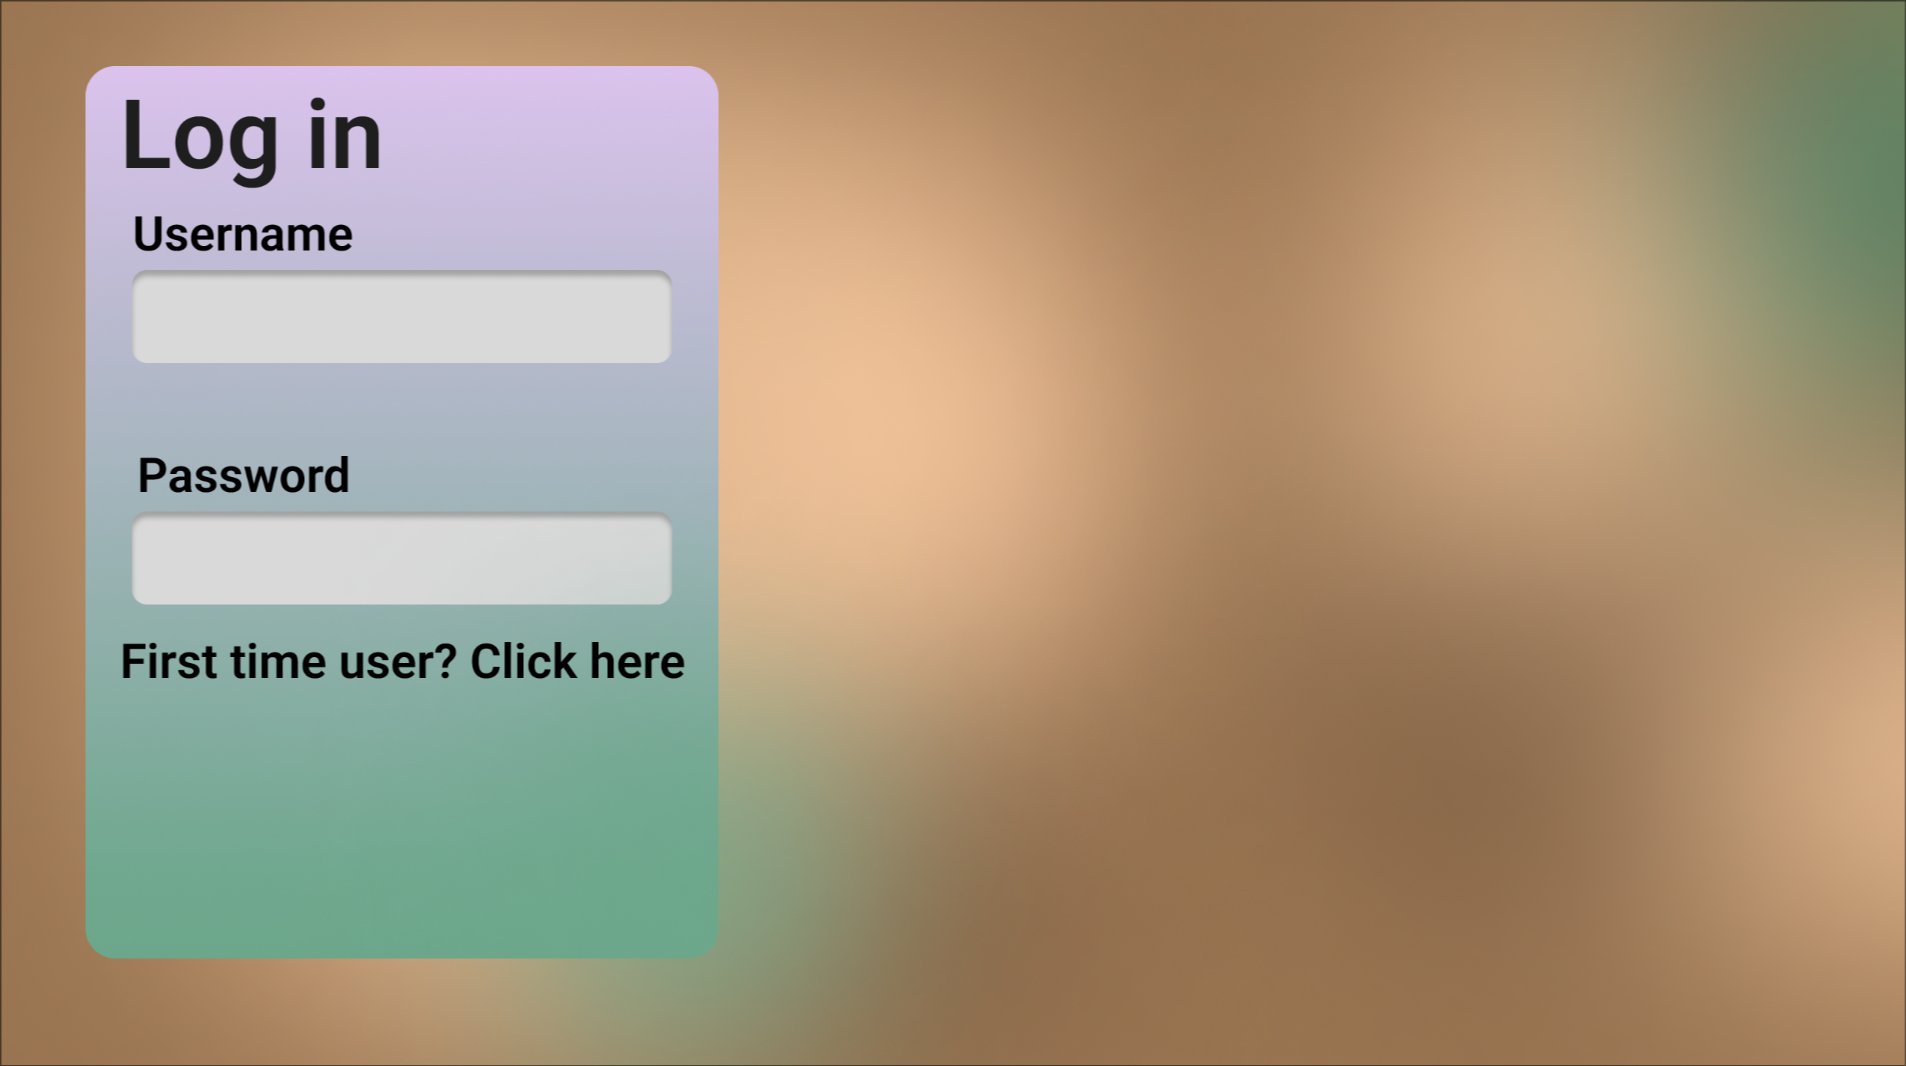
\includegraphics[scale=0.2]{Images/Log_In_UI.png}

\caption{Mock up of the log in/sign up page.}
\label{fig:login}
\end{figure}

\textit{Description:}
The log in/sign up page uses a brown aurora borealis inspired
background, with a purple and green log in box placed on the
left. Inside the log in box are 2 fields, username and
password, to allow the user to enter their credentials and 
log in. If it is their first time using the system then they 
can click on the link "First time user? Click here" which will
navigate the user to the account registration page and 
guide the user through how to create an account.
\\ \vspace{0.2cm}

\textit{Justification:}
Since our target userbase is the elderly I chose to display 
the text in a large and readable font, because it is quite 
likely that a good number of our users will have trouble 
with their eyesight. Consequently this means that our 
users shouldn't have problems with reading the text on our 
page. In the design I tried to create a nice design based on 
the colouring scheme that was outlined in section \ref{sec:ui}.
The design was chosen to create a professional look for the 
system as well as make the user feel calm and comfortable 
whilst on our website. In developing this calm theme 
throughout the design of our application we hope that 
the user will feel that our system is comfortable and 
reliable so that we hence provide a strong enough
motivating factor to encourage the user to switch from
the old system to our system.

\subsubsection{Help pdf document}

\begin{figure}[H]
\centering

\frame{
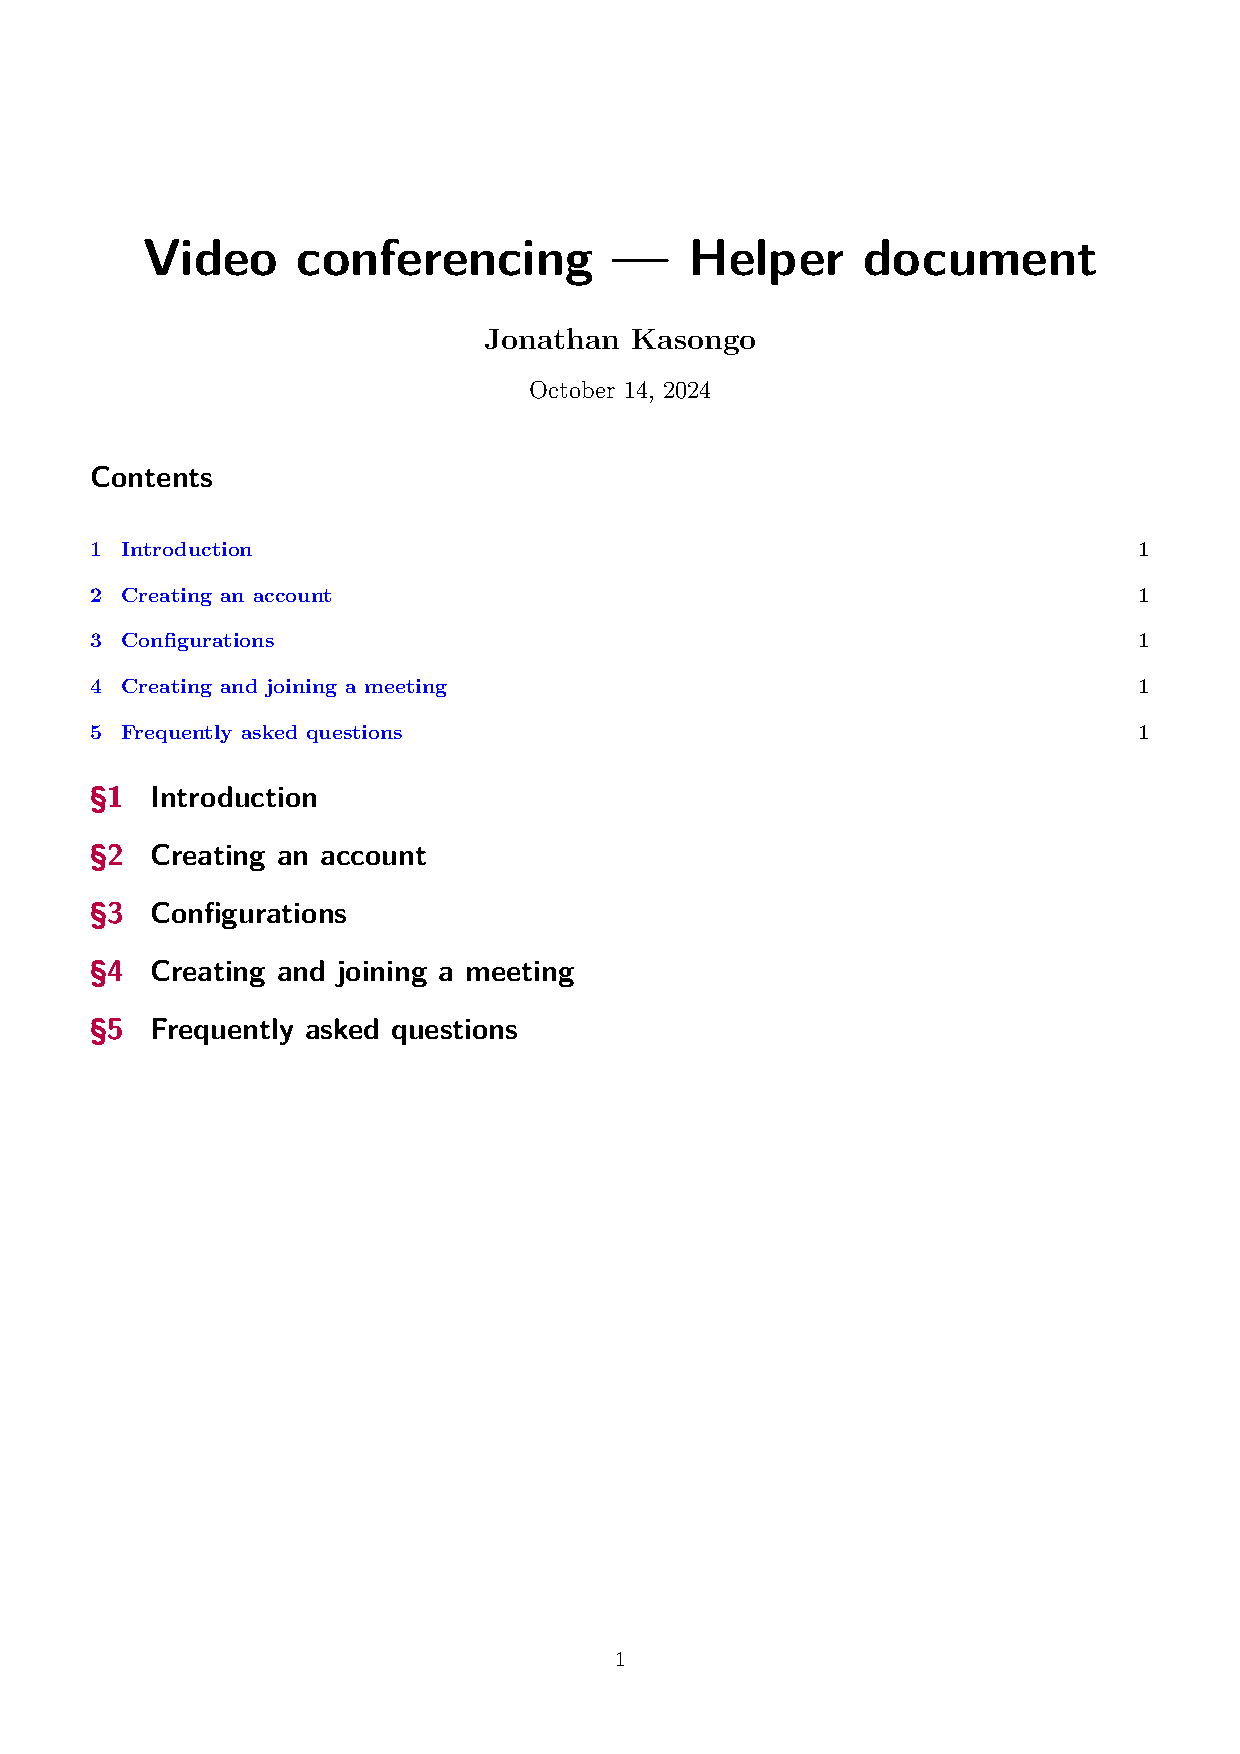
\includegraphics[height=9cm 
]{Help_Doc/Help_demo.pdf}}

\caption{Mock up of the helper document.}
\label{fig:help}
\end{figure}

\textit{Description:} The figure above presents the mock up 
that was created for the helper document that will be 
created along with this system. The document follows roughly
the same formatting as the one in this report, and has been 
split into 5 primary sections each providing a guide on how 
to use one portion of the software. Finally at the end of
the document we add a frequently asked questions section 
(FAQ) to put answers to common questions that our user may 
have regarding how to use the system.
\\ \vspace{0.2cm}

\textit{Justification:}
On the helper document we have chosen to stick with the
style used in this report providing a consistent and 
familiar theme to our users. The blue section links 
provide a quick way for our users to be able to navigate
to the sections that they specifically need. 
